\newcommand{\Constraints}[1]{\mathsf{constraints}({#1})}
\newcommand{\Frac}[1]{\mathsf{frac}({#1})}
\newcommand{\Addtimer}[4]{\mathsf{addtimer}({#1,#2,#3,#4})}

\section{From timed to untimed learning}  
\label{algorithm}
In this section, we consider another instance of Angluin's MAT framework.
Again, the teacher knows an MMT $\M$ but now the learner poses membership queries
to learn the \emph{untimed} behaviors of $\M$, and if an equivalence query fails then the counterexample is an \emph{untimed} behavior of $\M$.
We will show how an untimed teacher for MMTs can be implemented using a timed teacher.

\subsection{An untimed MAT framework for MMTs}
\label{sec:untimed-mat}
Given the equivalence of the timed and the untimed semantics of MMTs, it is natural to also 
consider an untimed setting, in which a learner tries to construct an MMT based on membership queries for untimed behaviors.

\todofv{Move canonical forms to section on untimed semantics?}
In the untimed framework, the teacher does not reveal the names of the timers of $\M$. 
It brings untimed behaviors into a ``canonical'' form, so that a learner can only observe these behaviors up to isomorphism.
Let us formalize this idea.
Suppose $\beta$ be an untimed behavior in which transitions update at most one timer.
We say that $\beta$ is in \emph{canonical form} if, for each $j$, the timer that is updated in the $j$-th event
(if any) is equal to $x_j$.
For each untimed behavior $\beta$ in which transitions update at most one timer, there is a unique untimed behavior
$\beta'$ in canonical form that is isomorphic to $\beta$.
We write $\can{\beta}$ to denote this $\beta'$.
\todofv{Add example}

Consider an untimed behavior $\beta$ in canonical form:
\begin{eqnarray*}
\beta & = & X_0 \xrightarrow{i_1/o_1, \rho_1} X_1  \cdots \xrightarrow{i_k/o_k, \rho_k} X_{k}.
\end{eqnarray*}
Let $1 \leq l \leq j \leq k$, $d \in \natplus$ and suppose that 
(1) $\rho_l$ either starts no timer or sets $x_l$ to $d$,
(2) $\beta$ does not contain a timeout event $\toevent{x_l}$.
Then $\Addtimer{l}{d}{j}{\beta}$ is the untimed behavior obtained from $\beta$ by
replacing $\rho_l$ by the update $x_l := d$, and adding $x_j$ to the sets $X_l$ up to (and including) $X_j$.
%In the untimed behavior $\emptyset \xrightarrow{i/o,~ x:=1 } \{ x\} \xrightarrow{i/o,~ y:=60 } \{ x, y\}$, for instance, we may remove timer $x$
%and obtain $\emptyset \xrightarrow{i/o } \emptyset \xrightarrow{i/o,~ y:=60 } \{ y\}$.
%Similarly, we may remove the first use of timer $x$ in the untimed behavior 
%$\emptyset \xrightarrow{i/o,~ x:=1 } \{ x\} \xrightarrow{i/o,~ x:=5 } \{ x\} \xrightarrow{\toevent{x}/o} \emptyset$ and obtain
%$\emptyset \xrightarrow{i/o } \emptyset \xrightarrow{i/o,~ x:=5 } \{ x\} \xrightarrow{\toevent{x}/o} \emptyset$.
Write $\beta \sqsubseteq \beta'$ if $\beta'$ can be obtained from $\beta$ by zero or more applications of function $\mathsf{addtimer}$.
Observe that $\sqsubseteq$ is a partial order with as minimal elements untimed behaviors in which every timer that is started also times out.
We call such untimed behaviors \emph{lean}.
We say that $\beta$ is a \emph{partial} untimed behavior of MMT $\M$ iff $\M$ has an untimed behavior $\beta'$ such that $\beta \sqsubseteq \beta'$.
\todofv{Add example}
%In the untimed framework, the teacher replies with partial untimed behaviors of $M$, brought in canonical form.

An \emph{untimed input word} over $I$ is a sequence $u = i_1 \cdots i_k$ over $\extinputs$ such that (1)
for all indices $j, l$, $i_j = \toevent{x_l}$ implies $l < j$, and (2) each timer occurs at most once in a timeout event.
The first condition  says that if a timer expires it must have been set in a previous event, and the second condition  expresses that
each timer may expire at most once.
Let $\beta$ be an untimed behavior in canonical form.
We can associate a unique input word $\untimedinputword(\beta)$ to $\beta$ by removing all the output events,
updates, and timer sets from $\beta$.
\todofv{Add example}
\begin{figure}
\begin{center}
 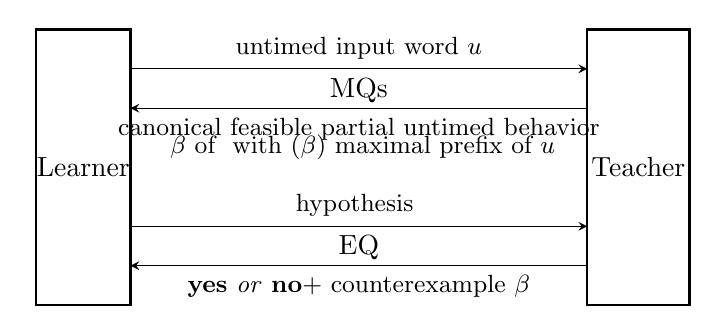
\begin{tikzpicture}[>=stealth]
            \draw [thick] (0,0) rectangle (1.2,3.5) node[midway] {Learner};
            \draw [thick] (7,0) rectangle (8.3,3.5) node[midway] {Teacher};
            \draw [->] (1.2,3) -- (7,3) node[midway,below] {MQs};
            \draw (1.2,3) -- (7,3) node[midway,above] {\small untimed input word $u$};
            \draw [<-] (1.2,2.5) -- (7,2.5) node[midway,below] {\small canonical feasible partial untimed behavior};
             \draw (4.15,2) node {\small $\beta$ of $\M$ with $\untimedinputword(\beta)$ maximal prefix of $u$};
            \draw [->] (1.2,1) -- (7,1) node[midway,below] {EQ};
            \draw (1.2,1) -- (7,1) node[midway,above] {\small hypothesis $\CH$};
            \draw [<-] (1.2,0.5) -- (7,0.5) node[midway,below] {\small {\bf yes} \emph{or} {\bf no}+ counterexample $\beta$};
        \end{tikzpicture}
\end{center}    
\caption{Untimed MAT framework}
\label{fig:untimed MAT}
\end{figure}

Our untimed learning setup, illustrated in Figure~\ref{fig:untimed MAT}, is similar to the timed setup:
again the teacher knows an MMT $\M$ and the learner initially only knows the set of inputs $I$ of $\M$.
Again, the learer may pose membership and equivalence queries.
But now a \emph{membership query} consists of an untimed input word $u$ over $I$.
The teacher replies with a maximal feasible partial untimed behavior $\beta$ of $M$ (in canonical form) such that
$\untimedinputword(\beta)$ is a prefix of $u$.
With an \emph{equivalence query}, the learner asks if a hypothesis $\CH$ with inputs $I$ is correct.
Upon receiving $\CH$, the teacher answers \emph{yes} if $\CH \approx_{\mathit{untimed}} \M$.
Otherwise it answers \emph{no} and supplies a counterexample, which now is a feasible untimed behavior $\beta$ (in canonical form) that
is a partial untimed behavior of $\M$ but not of $\CH$ (by Lemma~\ref{not untimed} such a counterexample exists).

\newcommand{\Zone}[1]{\mathsf{Zone}({#1})}

\subsection{Zones and constraints}

In order to implement an untimed teacher using a timed teacher, we need some basic facts and algorithms to
analyse and manipulate untimed behaviors and timed words that we will discuss in this subsection.

%It is not difficult to translate an MMTs to a timed automaton \cite{AD94,BengtssonY03} that accepts the same timed words.
%Through such a translation, verification and analysis tools for timed automata, such as Uppaal \cite{Uppaal4.0}
%become available for MMTs.
%MMTs are less expressive than timed automata. MMTs, for instance, do not contain time deadlocks or zeno loops that
%may prevent time from progressing.

MMTs have infinitely (in fact even uncountably) many configurations and it is thus necessary to use symbolic representations
for reachability analysis. Given an untimed behavior $\beta$ we want to compute its effect on a set of valuations. 
If $\beta =X_0$ and $K \subseteq\Vals{X_0}$ then we define $\Post_{\beta}(K) = K$.
If $\beta = X_0 \xrightarrow{i_1/o_1, \rho_1} X_1$ and
$K \subseteq\Vals{X_0}$ then $\Post_{\beta}(K)$ is equal to the set of all valuations $\tvals'' \in\Vals{X_1}$ such that
\[
  \exists \tvals \in K \exists d >0 \exists \tvals' \in\Vals{X_0} :
 \tvals \xrightarrow{d} \tvals' \xrightarrow{i_1/o_1, \rho_1} \tvals'' .
\]
The definition of $\Post_{\beta}(K)$ is extended inductively to arbitrary $\beta$ by 
$\Post_{\gamma \cdot \gamma'}(K) = \Post_{\gamma'} (\Post_{\gamma}(K))$, where $\gamma \cdot \gamma'$ is the decomposition of
$\beta$ into an untimed behavior $\gamma$ of length one and an untimed behavior $\gamma'$.
We write $\Zone{\beta}$ as abbreviation for $\Post_{\beta}(\Vals{\Head{\beta}})$.
%
For any untimed behavior $\beta$, $\Zone{\beta}$ can be symbolically represented and computed using a Difference Bound Matrices (DBMs)
 \cite{Di89}, as the transition relations $\xrightarrow{d}$ and $\xrightarrow{i_1/o_1, \rho_1}$ can be decomposed 
into elementary operations on DBMs such as reset, conjunction, and delay successors \cite{BengtssonY03}.

%It is easy to see that an untimed behavior $\beta$ is feasible iff $\Zone{\beta} \neq \emptyset$.
%Since emptiness of DBMs is decidable, this allows us to compute whether or not $\beta$ is feasible.

The next technical lemma's are needed further on:

\begin{lemma}
\label{lemma: feasibility concatenation}
Suppose $\beta, \beta'$ are untimed behaviors such that
$\Zone{\beta} = \Zone{\beta'}$. Let $\gamma$ be any untimed behavior.
Then $\beta \cdot \gamma$ is feasible iff $\beta' \cdot \gamma$ is feasible.
\end{lemma}

\begin{lemma}
\label{lemma finitely many zones}
$\{ \Zone{\beta} \mid \beta \mbox{ feasible untimed behavior of } \M \}$ is finite.
\end{lemma}
\begin{proof}
All the sets $\Zone{\beta}$ can be represented using DBMs. An MMT only has a finite number of timers that can only be set to a finite number of integer values. Since in an MMT the values of timers can only decrease, only finitely many numbers may
appear in the DBM's that represent the sets $\Zone{\beta}$. Thus all the sets $\Zone{\beta}$ can be represented by a finite
collection of DBMs.
\end{proof}

%Let $\beta$ be a feasible untimed behavior and let $x \in X$ be a timer. Then we say that $x$ is \emph{expirable} after $\beta$
%if there exists a valuation in $\Zone{\beta}$ in which $x$ is minimal.
%
%\begin{lemma}
%Suppose $\beta$ is a feasible untimed behavior with $\Last{\beta} = Y$ and $Y \xrightarrow{\toevent{x}/o, \rho} Y'$ is an untimed behavior.
%Then $x$ is expirable after $\beta$ iff $\beta \xrightarrow{\toevent{x}/o, \rho} Y'$ is feasible.
%\end{lemma}

Suppose that $\beta$ is an untimed behavior in canonical form:
\begin{eqnarray*}
\beta & = & \emptyset \xrightarrow{i_1/o_1, \rho_1} X_1  \cdots X_{k-1} \xrightarrow{i_k/o_k, \rho_k} X_k.
\end{eqnarray*}
We associate to $\beta$ a set of constraints with real-valued variables $t_1 ,\ldots t_k$ that denote the time of
occurrence of events $i_1 ,\ldots, i_k$ respectively. We add the following constraints to this set $\Constraints{\beta}$:
\begin{itemize}
\item
$0 < t_1 \leq d_{\max}$,
\item
for each index $j < k$:  $0 <  t_{j+1} - t_j \leq d_{\max}$,
\item
for each timeout event $i_j = \toevent{x_l}$: $t_j = t_l + \rho_j(x_l)$,
\item
for each clock $x_l$ that is started but does not timeout: $t_j \leq t_l + \rho_j(x_l)$,
where $j$ is the largest index such that $x_l \in X_j$, and
\item
for each pair of distinct indices $j$ and $l$ with $i_j, i_l \in I$: $\Frac{t_j} \neq \Frac{t_l}$ 
(to express that the fractional parts of $t_j$ and $t_l$ are different).
\end{itemize}
Note that $\beta$ is feasible iff the set of constraints $\Constraints{\beta}$ is satisfiable.
We may use an SMT solver to decide whether $\Constraints{\beta}$ is satisfiable and to compute\footnote{If an SMT solver
does not support fractions, we may compute a solution without these constraints and then use the wiggling approach
of Section~\ref{section untimed semantics} to ensure that the fractional times of inputs are different.} a solution.
\todofv{Add example}

\todofv{Move next lemma to earlier section}

\begin{lemma}
\label{not timed}
Suppose $\M, \N$ are MMTs with $\M \not\approx_{\mathit{timed}} \N$.
Then there exists a transparent timed word $w$ of $\M$ that is not a timed word of $\N$.
\end{lemma}

%\marginpar{What is the complexity of deciding eg timed equivalence or reachability of MMTs?}


%Note that for an untimed behavior $\beta$, the set $\zone{\beta}$ of valuations that can be reached with a timed behavior $\sigma$ with %$\untime(\sigma) = \beta$ can be symbolically represented using DBMs \cite{Di89}.
%We can do this since the transition relations $\xrightarrow{d}$ and $\xrightarrow{i_1/o_1, \rho_1}$ can be decomposed 
%into elementary operations on DBMs such as reset, conjunction, and delay successors \cite{BengtssonY03}.
%This allows us to compute whether an untimed behavior $\beta$ is feasible ($\zone{\beta}$ is empty), and
%whether a timer $x$ may expire after $\beta$ ($\zone{\beta}$ contains a valuation in which $x$ is minimal).

\subsection{Building an untimed teacher from a timed teacher}
We will now show how to construct an adapter that transforms a teacher for the timed setting into a teacher for the untimed setting.
The adapter maintains an integer variable $d_{\max}$ to store an estimate of the maximal timeout value that occurs in $\M$. Initially, the
adapter sets $d_{\max}$ to an arbitrary value, which may be increased based on the (transparent) timed words that it receives from
the timed teacher.

Suppose the untimed teacher receives a membership query, consisting of an untimed input word
$u = i_1 \cdots i_k$.
By induction on the length of $u$, 
we construct a response for $u$, that is, a feasible partial untimed behavior $\beta_k$ of $\M$ (in canonical form)
with $\untimedinputword(\beta_k)$ a maximal prefix of $u$.
If $k=0$, then response $\beta_0$ is the trivial partial untimed behavior $\emptyset$.
For the induction step, suppose that $k>0$.
Let $\beta_{k-1}$ be the response for $i_1 \cdots i_{k-1}$.
If $\beta_{k-1}$ contains less than $k-1$ inputs, then response $\beta_k$ is equal to $\beta_{k-1}$.
Now assume that $\beta_{k-1}$ contains $k-1$ inputs. We consider two cases:
\begin{enumerate}
\item
$i_k \in I$. Set $\beta := \beta_{k-1} ~ i_k ~ \omega ~ \emptyset$, where $\omega \in O$ is an arbitrary output that acts as placeholder.
Since $\beta_{k-1}$ is feasible (by induction hypothesis), it follows by Lemma~\ref{feasible plus input is feasible} that
$\beta$ is also feasible.
Thus the constraints in $\Constraints{\beta}$ are satisfiable and we may compute a solution $t_1 ,\ldots, t_k$.
Let $o_1 ,\ldots, o_{k-1}$ be the outputs occurring in $\beta_{k-1}$. Then
$w = t_1 ~ i_1 ~ o_1 ~ t_2 - t_1 ~ i_2 ~ o_2 ~ t_3- t_2 \cdots t_k - t_{k-1} ~ i_k ~ \omega$ is a transparent timed word.
Let $u' = \timedinputword(w)$ be the transparent timed input word associated to $w$.
We forward membership query $u'$ to the timed teacher.
Let $w'$ be the response from the timed teacher.
If $w'$ and $w$ are equal, except possibly for the last output symbol, which is $o_k$ in $w'$,
the response $\beta_k$ is equal to $\beta_{k-1} ~ i_k ~ o_k ~ \emptyset$.
Otherwise, $w'$ contains some timeout event that was not supposed to happen according to untimed input word $u$.
Since $u'$ is transparent, $w'$ is transparent as well. Thus we may extract from $w'$ which event $l$ started the timer, to which value
$d$ the timer was set, and the index $j$ of the timeout event.
We set $\beta_{k-1} := \Addtimer{l}{d}{j-1}{\beta_{k-1}}$ and perform step (1) again. 
Note that the number of iterations is finite.
\item
$i_k = \toevent{x_l}$, for $l < k$.
If $\beta_{k-1}$ assigns value $e$ to timer $x_l$ then
we set $\beta := \Addtimer{l}{e}{k-1}{\beta_{k-1}} ~ \toevent{x_l} ~ \omega ~ \emptyset$ and check whether $\Constraints{\beta}$ is
satisfiable. If not then response $\beta_k$ is equal to $\beta_{k-1}$.
If $\beta_{k-1}$ does not assign a value to $x_l$ then define, for $1 \leq e \leq d_{\max}$,
$\beta^e = \Addtimer{l}{e}{k-1}{\beta_{k-1}} ~ \toevent{x_l} ~ \omega ~ \emptyset$.
Search for the smallest $e$ for which $\Constraints{\beta^e}$ is satisfiable and set $\beta := \beta^e$.
If there is no such $e$ then response $\beta_k$ is equal to $\beta_{k-1}$.
Otherwise, we compute a solution $t_1 ,\ldots, t_k$ for $\Constraints{\beta}$.
Let $o_1 ,\ldots, o_{k-1}$ be the outputs occurring in $\beta_{k-1}$. Then
$w = t_1 ~ i_1 ~ o_1 ~ t_2 - t_1 ~ i_2 ~ o_2 ~ t_3- t_2 \cdots t_k - t_{k-1} ~ \toevent{x_l} ~ \omega$ is a transparent timed word.
Let $u' = \timedinputword(w)$ be the transparent timed input word associated to $w$.
We forward membership query $u'$ to the timed teacher.
Let $w'$ be the response from the timed teacher. Since $u'$ is transparent, $w'$ is transparent as well.
If $w'$ and $w$ are equal, except possibly for the last output symbol, which is $o_k$ in $w'$,
the response $\beta_k$ is equal to $\beta$ with the last output set to $o_k$.
It may also occur that, even though the last event of $w'$ is a timeout triggered by event $i_l$, the value $e'$ to which this timer is
set is different from $e$. In this case response $\beta_k$ is set to
$\beta_k = \Addtimer{l}{e'}{k-1}{\beta_{k-1}} ~ \toevent{x_l} ~ o_k ~ \emptyset$, where $o_k$ is the last output in $w'$.
Finally, it may occur that $w'$ contains some timeout event that was not supposed to happen according to untimed input word $u$.
In this case, we extract from $w'$ which event $l$ started the timer, to which value
$d$ the timer was set, and the index $j$ of the timeout event.
We set $\beta_{k-1} := \Addtimer{l}{d}{j-1}{\beta_{k-1}}$ and perform step (2) again. 
Again the number of iterations is finite.
\end{enumerate}
\todofv{Add example!}
%\paragraph{Example}
%Consider a scenario where the timed teacher knows the MMT of Figure~\ref{fig:nondeterminism} (bottom).
%Suppose that $d_{\max} = 5$ and the untimed teacher receives a query for input word $i ~ i$. The adapter starts with defining
%\[
%\beta_0 = \emptyset
%\]
%Next it solves $\Constraints{\emptyset ~ i ~ \omega ~ \emptyset} = \{ 0 < t_1 \leq 5 \}$.
%Suppose it arrives at the solution $t_1 = 1$. Based on this, the timed input word $1 ~ i ~ 0$ is
%forwarded to the timed teacher. The timed teacher responds with $1 ~ i ~ o$ and the adapter defines
%\[
%\beta_1 = \emptyset ~ i ~ o ~ \emptyset
%\]
%The constraints in $\Constraints{\emptyset ~ i ~ o ~ \emptyset ~ i ~ \omega ~ \emptyset}$ are still trivial.
%Suppose adapter finds solution $t_1 = 1,~ t_2 = 4.1$ and forwards timed input word  $1 ~ i ~ 3.1 ~ i ~ 0$ to the timed teacher.
%Based on the response $1 ~ i ~ o ~ 2 ~ \mathit{to} ~ o$, the adapter realized that the first transition starts a timer
%and solves $\Constraints{\emptyset ~ i,x:=1 ~ o ~ \{ x \} ~ i ~ \omega ~ \emptyset}$.

Implementing equivalence queries is easy.
Suppose that the untimed teacher receives an equivalence query $\CH$.
Then we just forward this query to the timed teacher.
If the timed teacher answers \emph{yes} then $\CH \approx_{\mathit{timed}} \M$.
In this case, by Theorem~\ref{timedimpliesuntimed}, $\CH \approx_{\mathit{untimed}} \M$,
and thus the untimed teacher should also return the result \emph{yes}.
If the timed teacher answers \emph{no} and returns a counterexample $w$,
then $w$ is a transparent timed word of $\M$ but not of $\CH$.
In this case, by Theorem~\ref{untimedimpliestimed}, we may conclude that
$\CH \not\approx_{\mathit{untimed}} \M$, and thus the untimed teacher should also return a result \emph{no}.
Since $w$ is a transparent timed word of $\M$, it 
follows by Lemma~\ref{lemma unique causality map} that $w$ 
has a unique causality map $c$.
This allows us to transform $w$ into a feasible untimed behavior $\beta$ (in canonical form) that is a partial untimed
behavior of $\M$ but not of $\CH$: the causality map tells us exactly which timers are set and timeout. 
Thus the untimed teacher may return $\beta$ as counterexample.
If our estimate $d_{\max}$ of the maximal timeout value of $\M$ is too low, then it may occur that in $w$ the timeout value of some
timer is larger than $d_{\max}$. In this case, the value of $d_{\max}$ is updated to the newly observed maximal timeout value.
\todofv{Think through implications of updating $d_{\max}$.}





